\chapter{Evaluation}
\label{chap:evaluation}
In this chapter, we evaluate our approach. The evaluation was done using the simulator described in the previous chapter.

When evaluating our approach we took into consideration multiple metrics that we considered the most relevant for the proposed approach, namely:

\begin{itemize}
	\item \textbf{Percentage of committed transactions} This metric measures the percentage of transactions committed during the simulation. This metric is important because since we are effectively lowering the number of nodes that know of a transaction we wanted to make sure that in our approach transactions would not get lost in the dissemination process. Hence this metric measures the resilience of the system, meaning that if our protocol is not able to commit the same amount of transactions as the base protocol then it is not resilient enough;
	\item \textbf{Commit time} This metric measures the commit time of transactions. The commit time is the time it takes for a transaction to appear in a block since it was created. This metric is also very susceptible to changes to the protocol especially changes like the ones we are proposing since they are extremely connected with the dissemination of information. Furthermore, making sure this metric does not cross critical values (30 minutes) is also essential for our approach to be even considered one day to be integrated into the Bitcoin client. Hence, this metric is one of the indicators of the performance of our protocol, our objective when measuring this metric is to make sure that at least we maintain the same commit time;
	\item \textbf{Amount of messages sent} This metric measures the amount of messages exchanged in the network. This metric is very important because it will determine if our approach brings anything of value to Bitcoin as this is the main metric we want to have an impact on by lowering it. This metric is the one where we want to observe the biggest improvement if our protocol works properly;
	\item \textbf{Amount of information sent} This metric measures the amount of information exchanged in the network. We did not expect an improvement in this metric as significative as in the metrics "Amount of messages sent" because the size of the messages exchanged is small.  
\end{itemize}

This chapter is divided into two sections, Section~\ref{sec:sim_tuning} that details how we tuned our simulator in order for it to be as faithful as possible to Bitcoin. Then in Section~\ref{sec:results} we will go over the results we obtained and discuss them. Finally, Section~\ref{sec:evsum} summarises the results obtained.

\section{Simulator Tuning}
\label{sec:sim_tuning}
To tune the simulator we used the metrics that we had gathered from websites like \url{blochain.info} and \url{bitnodes.earn.com} and from our modified client, but we also tuned the simulator experimentally by comparing results we were obtaining by running the base protocol with the real Bitcoin client. We considered that all nodes were running a version of the Bitcoin core client that implements compact blocks. Blocks are always relayed through compact block unless the neighbour does not possess the previous block. When a node receives a transaction it will always relay it unless that node is Byzantine. Nodes can not have more than 125 connections. When a node tries to establish a connection with another node, the other node will always accept it. The network model that we used in the experiments of Section~\ref{sec:results} were composed solely of nodes that followed the protocol accordingly.

Due to the complexity of the protocol, simulating the full network resulted in resource intensive simulations that lasted for days.
%Running simulations of big Bitcoin networks in a language not optimised for efficiency resulted in the simulations being very demanding in terms of computations and space required which resulted in the simulations taking a long time (scale of days) to complete.
To overcome this, we scaled down the size of the simulated network as follows.
First, we ran the original protocol with 6000 nodes and with 625 nodes and compared the metrics discussed below. The results we obtained were equivalent for both network sizes hence, for the rest of this section we consider a network size of 625 nodes. This proportional scaling between 6000 nodes (size registered when we started experimenting) and 625 nodes, allowed us to quickly explore different possible solutions and run multiple instances of each test. The results presented are an average of 3 independent runs that correspond to 34 hours in real time. We discarded the first and last 5 hours of each run in order to study the system in a stable state. 

\section{Results}
\label{sec:results}
We started by exploring the different possible solutions to reduce network usage without having a negative impact on the system. In all experiments below, we use the following notation: \textsl{Tn} where n specifies the value of the variable \textsl{max\_t\_nodes}; and \textsl{Rn} specifies the value of the variable \textsl{max\_r\_nodes} present in the previous algorithms. Note that for these experiments we did not used Algorithm~\ref{alg:inc} because we wanted to manually determine the best values for the aforementioned variables.

Hence, this section is divided into two subsections in the Section~\ref{sec:sri} we will present the results of the experiments and how we determined the best possible configuration for the variables \textsl{max\_t\_nodes}, \textsl{max\_r\_nodes} and \acrshort{ip}. After in Section~\ref{sec:ea} we will present the results of running Agorithm~\ref{alg:inc} together with the rest of our solution and study its abilities to converge to the optimal configuration found manually.

\subsection{Skewed Relay Impact}
\label{sec:sri}
Initially we tested with multiple combinations of $n={1,2,3,4}$ for both \textsl{T} and \textsl{R}. After these preliminary experiments, we observed that for values of $n={3,4}$ the results were practically the same as the results without our approach. However, with $n={1,2}$ we observed a considerable reduction in the number of duplicated advertisements.
These results also support our logs in the real client, where the average number of duplicates was 6.6. With this in mind, for the rest of the experiments, we considered only the combinations of: \textsl{T2\_R2; T2\_R1; T2\_R0; T1\_R1; T1\_R0}. Additionally, for each configuration, we also experimented with both values of the variable \textsl{\acrshort{ip}}.

\begin{figure}[h]
\centering
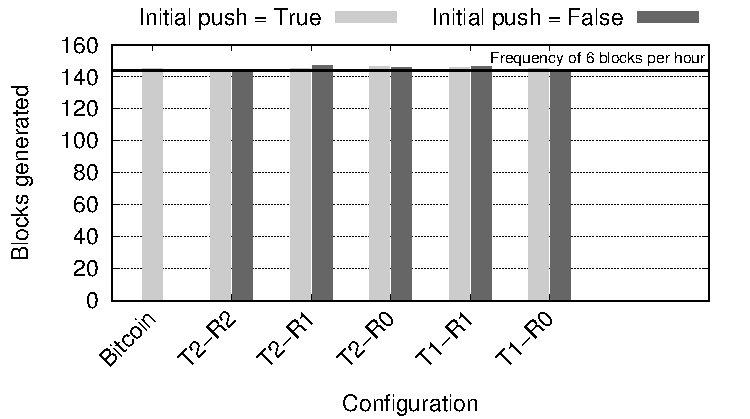
\includegraphics[width=0.7\textwidth]{plots/blocks-gen.pdf}
\caption{Blocks generated.}
\label{fig:nb-blocks}
\end{figure}

\begin{figure}[h]
\centering
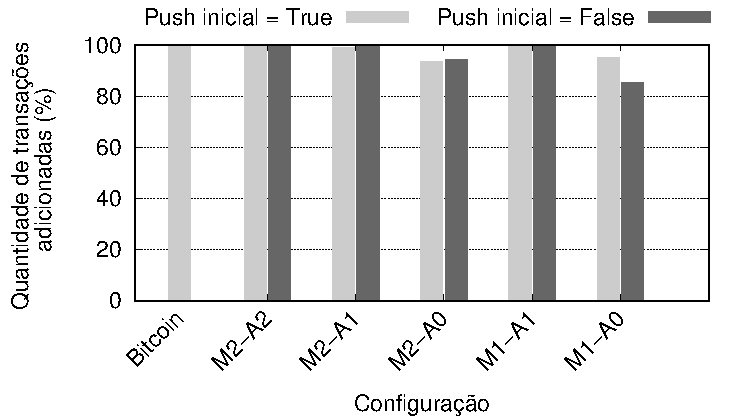
\includegraphics[width=0.7\textwidth]{plots/tx-added.pdf}
\caption{Percentage of transactions committed.}
\label{fig:tx-added}
\end{figure}

Figure~\ref{fig:nb-blocks} shows, for each configuration, the amount of blocks that were generated during each experiment, while Figure~\ref{fig:tx-added} shows the percentage of transactions added to blocks throughout the multiple configurations. As it is possible to observe, the simulation generated for all configurations the expected amount of blocks for a day ($\approx 144$) and committed all the created transactions (100\%). From these results we can conclude two things. The first is that we configured our simulator properly as all simulations generated the expected amount of blocks per day, the second conclusion is that all the configurations tested were resilient enough to commit all the transactions generated. This means that both Algorithm~\ref{alg:class} and Algorithm~\ref{alg:diss} are working properly as nodes are ranking neighbours properly and their transactions are reaching at least a miner which adds them to a block. However, we still need to check the performance of the metric commit time to draw conclusions on which is the best configuration.

\begin{figure}[h]
\centering
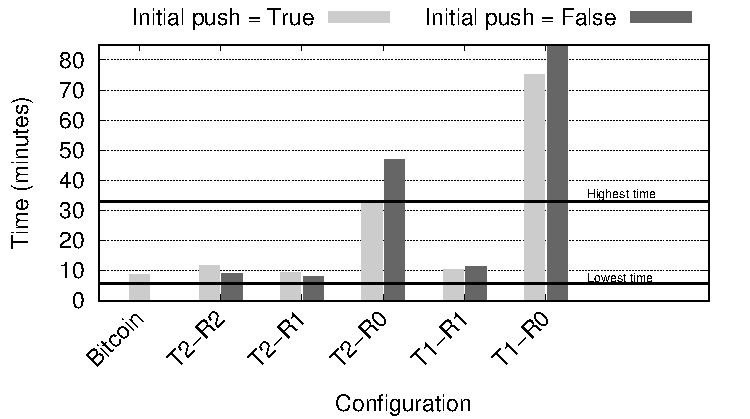
\includegraphics[width=0.7\textwidth]{plots/commit-time.pdf}
\caption{Average time it takes for a transaction to be committed.}
\label{fig:commit-time}
\end{figure}

Regarding the commit time Figure~\ref{fig:commit-time} shows the average transaction commit time for each configuration.
The horizontal lines represent the highest and lowest average time it took for a transaction to be committed in Bitcoin. 
In this image, we can clearly see that both configurations \textsl{T2-R0} and \textsl{T1-R0} are not good enough to achieve a commit time comparable to Bitcoin. This increase in the average commit time happens because although transactions are reaching miners they are not reaching the miner that is going to mine the next block. Another factor that contributes to this is that some cluster of nodes will all send their transactions to the same node.  This shows that sending transactions for at least one random node alongside the top nodes has a great impact in the commit time as previously discussed in Section~\ref{sec:sr}.

With this, both configurations are not eligible anymore for best configurations as a low commit time is one of the most important aspects of a cryptocurrency.

\begin{figure}[h]
\centering
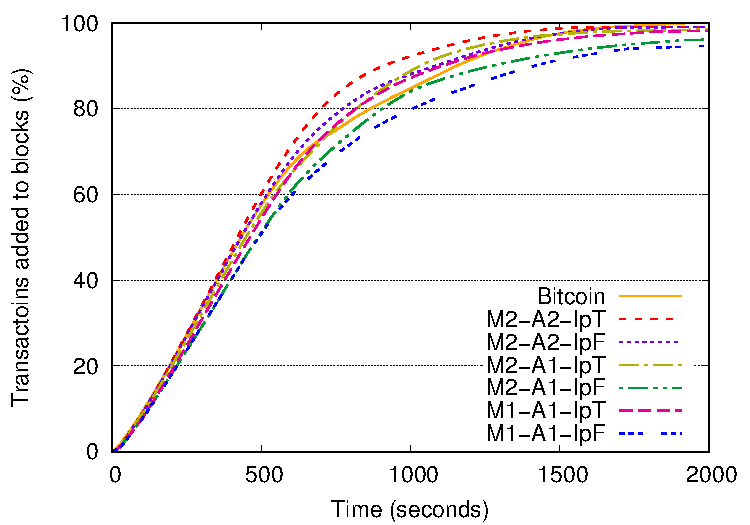
\includegraphics[width=0.7\textwidth]{plots/cdf_commit.pdf}
\caption{Cumulative distributed function of the time it takes for a transaction to be committed.}
\label{fig:cdf-commit}
\end{figure}

Figure~\ref{fig:cdf-commit} shows the cumulative distributed function of the time it took to commit all the transactions, hence, it is a different perspective of Figure~\ref{fig:commit-time}. 
From both figuress, we can also conclude that sending a new transaction to all the neighbours (\emph{ip=T}) has a very low impact in the time it takes to commit a transaction. We attribute this to the fact that the time it takes for a transaction to reach all the miners is orders of magnitude (few seconds versus dozen of minutes) lower than the rate at which blocks are being generated. Therefore we can already exclude the configuration with (\emph{ip=T}) as those configurations will always generate more messages than the other configurations without providing any major improvement in the other metrics.

With the impact of each configuration in the transaction commit time and number of transactions analysed, we now focus on the impact on reducing network usage.

\begin{figure}[h]
\centering
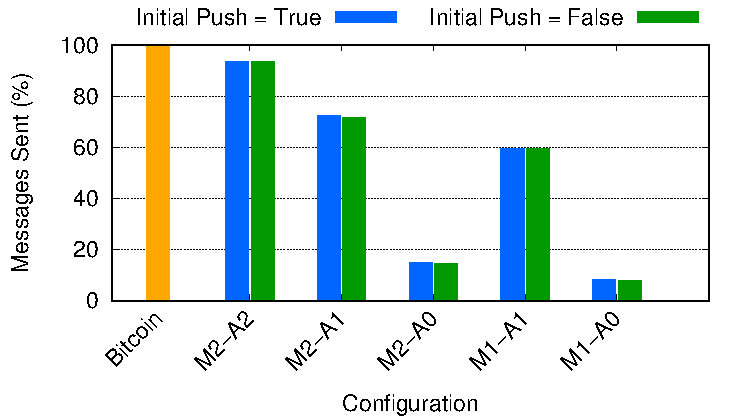
\includegraphics[width=0.7\textwidth]{plots/msg-sent.pdf}
\caption{Total number of messages sent.}
\label{fig:msg-sent}
\end{figure}

\begin{figure}[h]
\centering
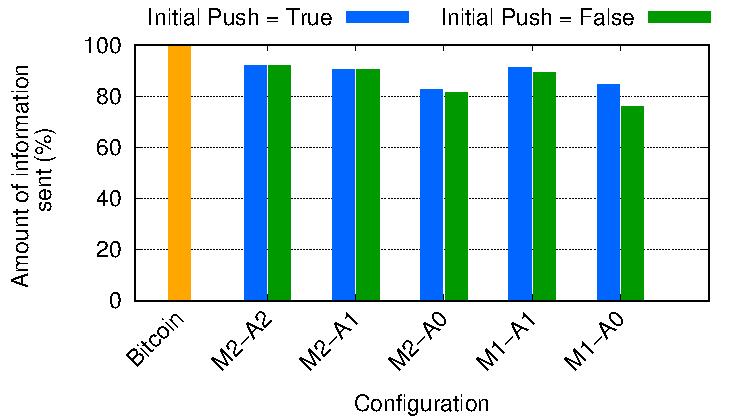
\includegraphics[width=0.7\textwidth]{plots/mb-sent.pdf}
\caption{Amount of information sent.}
\label{fig:mb-sent}
\end{figure}

Figure~\ref{fig:msg-sent} shows ratio between the total number of messages sent in each configuration to the same amount in the Bitcoin network. As expected, the configurations with a higher amount of savings were the configurations that did not relay to random nodes. This happens because when we send a transaction to a random node there is a higher chance that that node still does not have that transaction and will request it. Unfortunately, as we have seen previously, both these configurations are not viable because both take very long to commit transactions. Figure~\ref{fig:mb-sent} shows a different perspective by depicting the savings in the total amount of information transmitted which, as expected, follows a similar pattern to Figure~\ref{fig:msg-sent}. We can also see that the savings from Figure~\ref{fig:mb-sent} are not as big as the ones from Figure~\ref{fig:msg-sent}.
This happens because the advertise messages that we avoid sending are not very big in size. However, processing those spurious incurs an additional cost to the nodes.

By analysing these results, we can conclude that the most promising configuration is \textsl{T1-R1} with \textsl{ip=False} because not only it achieves relevant savings (reduction in the number of messages sent in 41.5\% and reduction of the amount of information sent in 10.2\%) but also it preserves the properties of the original Bitcoin.

\subsection{Adaptation}
\label{sec:ea}

In the previous experiments, and to determine the best possible configuration we used a stable network, where miners were always the same nodes. However, as any large network, Bitcoin is prone to changes.
We now study the adaption policy introduced in Algorithm~\ref{alg:inc}.
Initially, all nodes send advertisements to \textsl{T = neighbourhood / 2} and \textsl{R = neighbourhood / 2} which is the same as sending advertisements to all their neighbours as in the regular Bitcoin. Then throughout the simulation, the algorithm will progressively determine the best \textsl{Tn-Rn} configuration for each node by either increasing or decreasing both variables. We performed three experiments, one where we did not make any changes to the network, another where we change two miners in the network at 12 hours into the simulation and finally a third one where we changed all the miners at 12 hours into the simulation. With these experiments, we want to determine if our solution is able to adapt to the network changes and preserve the commit time while still sending as few messages as possible. These experiments were run for a simulation time of 58 hours in order so see if the system would stabilise after the miners being changed.

\begin{figure}[h]
\centering
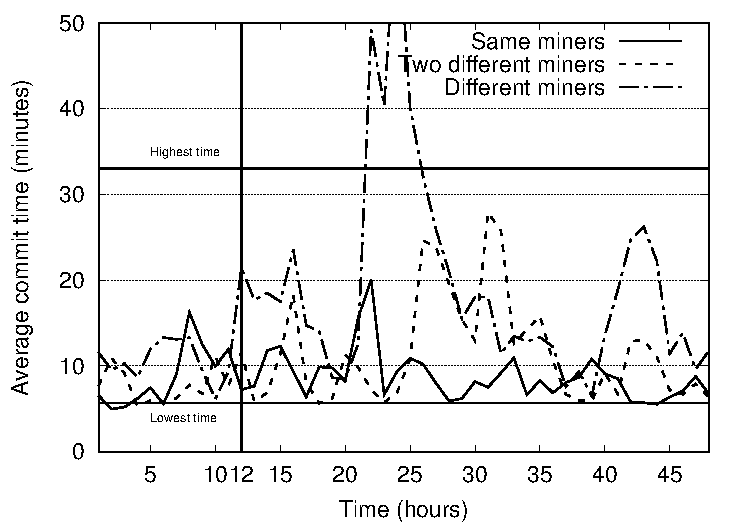
\includegraphics[width=0.7\textwidth]{plots/commit_over_time.pdf}
\caption{Average commit over time.}
\label{fig:commit-over-time}
\end{figure}

Figure~\ref{fig:commit-over-time} shows the average commit time over the period of time simulated. It also shows the two horizontal lines that were in Figure~\ref{fig:commit-time}, delimiting the minimum and maximum observed Bitcoin commit times. 

This figure has three lines one for each of the configurations described previously. 
Starting with the line that represents the simulation where no miners were changed, we can see that for the majority of the time the commit time was pretty constants and that transactions were always committed in time. 
There is a moment where it peaked around 22 hours but that might have occurred due to some nodes lowering too much the size of \textsl{T and R}.

Regarding the line that represents the simulation where we changed two miners, it also behaves similarly to the previous line until around the 12th hour were then two miners were changed this produced a delayed peak between hours 14 and 17 and then at hours 24 to 35. The first peak was due to the change of miners and the second probably happened due to some nodes lowering too much the size of \textsl{T and R} which was then also aggravated by the change in miners. However is worth noting that both these peaks did not surpass the line of the highest time observed in Bitcoin.

Finally, for the line that represents the simulation where all the miners changed we can see that this line had a huge peak after the change of miners. This is because this scenario corresponds all current miners to stop mining and a new set of miners completely replacing them, which is very unlikely in practice. However, it is worth noting that in the end, all simulations started converging to the same commit that that we observed for the configuration \textsl{T1-R1} in Figure~\ref{fig:commit-time}.

\begin{figure}[h]
\centering
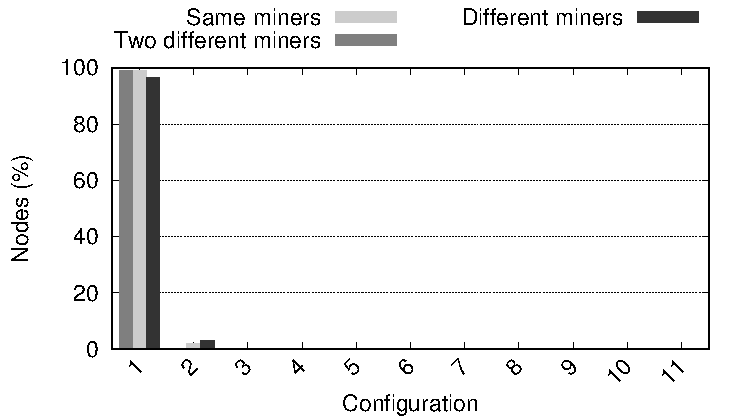
\includegraphics[width=0.7\textwidth]{plots/nodes_per_config.pdf}
\caption{Distribution of the nodes by the different possible configurations.}
\label{fig:node-per-conf}
\end{figure}

Figure~\ref{fig:node-per-conf} displays the percentage of nodes in each configuration at the end of the simulation for the three runs. In the \emph{y} axis is the percentage of nodes and in the \emph{x} axis are the multiple configurations observed in the simulation, for instance we can see that for the simulation were the miners were always the same that at the end of the simulation almost 100\% of the nodes were with a configuration \textsl{T1-R1} configuration 1 and that no nodes had the configuration \textsl{T11-R11} configuration 11. This image shows that in all three scenarios at the end almost all the nodes converged to the configuration that we had previously deemed ideal (\textsl{T1-R1}).

\section{Summary}
\label{sec:evsum}

We can drawn several interesting conclusions from these experiments.
First, we can see that if we are in the presence of a stable network, then our solution is going to start adapting to the network and converge to the configuration that we previously deemed ideal (\textsl{T1-R1}), as seen in Figure~\ref{fig:node-per-conf}. Secondly, we can conclude that if there are slight changes to the network, then the average commit time of our solution is going to slightly deteriorate, but eventually the algorithm will increase the size of \textsl{T} and \textsl{R} to cope with the changes and the average commit time will once again converge the values before the changes. Finally, if our solution is confronted with drastic changes to the network it will not be able to maintain the current commit time, given that at 12 hours into the simulation most nodes were configured to \textsl{T1-R1} which is not resilient enough for these cases.
We note however that such sudden shift in mining power is unlikely to happen.
Regardless, after some time our approach will start converging to the desirable stable configuration.


This chapter presented the experimental evaluation of our protocol, detailing experiments conducted in order to assess which was the best configuration of the variables \textsl{max\_t\_nodes} and \textsl{max\_r\_nodes}. In the best case, our protocol is able to save 41.5\% of the messages sent and 10.2\% of the information sent by the traditional Bitcoin protocol. We have also shown that our protocol is able to sustain changes in the network while still maintaining the performance of the current Bitcoin protocol.

%Note that in our experiments we configured the most desirable configuration to be the one where we send as few messages as possible (\textsl{T1-R1}) but if for instance, we wanted to maintain the commit time in very dynamic environments then the most desirable configuration would probably be \textsl{T2-R2} as it would be more resilient against dramatic changes.
